%!TEX root=../document2.tex

\section{Einleitung}
\label{sec:Einleitung}
Load Balancing ist kein neues Konzept im Server- und Netzwerkbereich. Viele Produkte, wie z.B. Router die Netzwerkverkehr über verschiedene Netzwerk Ressourcen zum gleichen Ziel verteilen, können unterschiedliche Arten des Load Balancing durchführen. Im Gegensatz zum Router wird bei Server Load Balancing der Netzwerkverkehr über verschiedene Server Ressourcen verteilt. Anfangs wurden Load Balancer als reine Lastenverteiler verwendet, doch heute sind Load Balancer schon so weit entwickelt, dass sie zusätzliche Funktionen wie Healthchecks, Optimierung von Datenflüssen, etc. zur Verfügung stellen.

Im Webhostingbereich wird Load Balancing typischerweise für die Verteilung von http-Verkehr auf mehrere Server (Nodes), die als Web Front-End agieren, eingesetzt. Der Load Balancer beurteilt die Antwortzeiten und Auslastung der einzelnen Server und verteilt basierend auf dieser Beurteilung die Anfragen. Durch die Verteilung des Dienstes auf mehrere Server schützt man sich zusätzlich vor Hardwareausfall, da bei Ausfall eines Server Nodes der Netzwerkverkehr einfach über andere Nodes erfolgen kann. Das primäre Ziel ist es, den Netzwerkverkehr bei hoher Nachfrage auf alle vorhandenen Nodes aufzuteilen, um die bestmögliche Performance zu gewährleisten. Der User weiß normalerweise nichts über vorhandene Backend- bzw. Backupserver, für ihn scheint es so als ob nur ein Server hinter einem Dienst steht. [1]

\subsection{Wann und wozu verwendet man Load Balancing?}
\label{sec:Wann und wozu verwendet man Load Balancing?}

\begin{list}{•}{}
\item Failover und Redundanz

	  Ein wesentliches Einsatzgebiet des Load Balancing ist die Ausfallsicherheit und die daraus resultierenden 		  erhöhte Uptime (Betriebszeit). Durch Verwendung von mehreren identischen Nodes kann der Netzwerkverkehr im 	  Falle eines Hardware oder Softwarefehlers umverteilt werden und die Website, Dienst, etc. bleibt 			 	  verfügbar. 
\item Wachsende Nachfrage und Verfügbarkeit
	  
	  Falls die Website, Dienst, etc. so beliebt wird, dass ein einziger Server die Masse an Anfragen nicht in 			  absehbarer Zeit abarbeiten kann (was zu z.B. lange Wartezeit bei Seitenaufbau führt), sollte man ebenfalls 	  Load Balancing einsetzten. Dadurch können die Anfragen auf mehrere Server verteilt werden und so ist die 			  Verfügbarkeit wieder gegeben. [1]     
\end{list}

\subsection{Beispiel Website}
\label{sec:Beispiel Website}
Anhand dieses kleinen Beispiels einer Website möchte ich die zwei oben genannten Haupteinsatzgründe für Load Balancing veranschaulichen. 

Mögliche Probleme bei einer Website: zu hohe Anzahl an Anfragen für Webserver (falls die Seite nur von einem Webserver gehostet wird), Datenbank- bzw. Webserver fällt aus  .

Lösung durch Load Balancing: Einsatz von mehreren Servern. Um für eine hohe Anzahl an Anfragen gerüstet zu sein, muss die Website über mehrere Webserver verfügbar sein. Da eine Domain nur einem physikalischen Server zugewiesen werden kann, wird der Load Balancer zwischen dem Internet und den Webservern geschaltet und bekommt die öffentliche Domain zugewiesen. Wenn mehrere User die Website abrufen, beurteilt der Load Balancer die Antwortzeiten und Auslastung der einzelnen Webserver und verteilt die Anfragen so, dass die bestmögliche Performance erreicht wird. Außerdem wird so auch die Ausfallsicherheit der Website gewährleistet, da die Website jetzt über mehrere Webserver gehostet wird. Zusätzlich wird in diesem Beispiel ein Backupserver der Datenbank erstellt. Falls der Datenbankserver ausfällt oder ausgetauscht werden muss, springt einfach der Backupserver ein.      

\subsection{Notwendigkeit von Load Balancing}
\label{sec:Notwendigkeit von Load Balancing}
Das primäre Ziel von Load Balancing ist es den Netzwerkverkehr bei hoher Nachfrage auf alle vorhandenen Nodes aufzuteilen, um die bestmögliche Performance zu gewährleisten. Netzwerke und Server sind die Hauptgründe, warum Load Balancing notwendig ist. In der heutigen Zeit, ist das Internet ein wichtiger Bestandteil für jedes Unternehmens ist (um Netzwerk zwischen Firma, Lieferanten, Kunden, etc. zu erzeugen), bei dem es auch um viel Geld geht. Firmen, vor allem im e-commerce Bereich (elektronischer Handel), können es sich nicht leisten, wenn ihr Netzwerk entweder sehr langsam ist bzw. ausfällt. 
Um z.B. eine Website für elektronischen Handel zu erstellen, muss man Faktoren wie Server, Switches, Firewalls, etc. berücksichtigen. Durch das Verwenden von mehreren Servern für so eine Website entstehen aber Herausforderungen in den Bereichen Skalierbarkeit, Verwaltbarkeit und Verfügbarkeit. Load Balancing löst zusätzlich viele dieser Probleme.

\textbf{Skalierbarkeit} \\

Skalierbarkeit ist kein neues Problem. Früher ist eine Applikation auf einem Server gelaufen. Falls dieser Server für die Applikation nicht mehr ausreichend war, wurde dieser entweder verbessert oder durch einen performanteren Server ersetzt. Durch Load Balancing ist es jedoch möglich, die Applikation auf mehreren Servern zu verteilen. Durch die mehreren Server ist es möglich, sämtliche Anfragen zu verteilen um bestmögliche Performance zu gewährleisten. Load Balancer verwenden Scheduling Algorithmen um die Anfragen zu verteilen. 

\textbf{Verwaltbarkeit} \\

Wenn die Serverhardware verbessert oder das Betriebssystem aktualisiertet werden muss, muss der Server abgeschaltet werden. Man kann das natürlich in der Zeit machen, in der am wenigsten Bedarf an der Website/Dienst besteht (vermutlich in der Nacht), jedoch hat man trotzdem eine Ausfallzeit (Downtime). Doch manche Firmen können sich überhaupt keine Ausfallzeit leisten oder haben konstanten Bedarf  an ihrem Service. Ein Load Balancer kann Server, die für Wartungszwecke offline gestellt werden müssen, ohne Downtime ausschalten. Das wird gewährleistet, in dem der Load Balancer keine weiteren Anfragen an diesen Server weiterleitet und wartet bis sämtliche bestehende Anfragen abgearbeitet wurden. Dann kann der Server offline gestellt werden. Sämtliche Anfragen werden auf die anderen Server weitergeleitet. Zusätzlich helfen Load Balancer beim Verwalten von Content Managementsystem, da es bei solchen Systemen ebenfalls sein kann, das ein Server nicht ausreicht.   

\textbf{Verfügbarkeit} \\

Der Load Balancer kontrolliert kontinuierlich die Verfügbarkeit aller Server und laufenden Applikationen. Wenn der Healthcheck einer dieser Server oder Applikationen scheitert, sendet der Load Balancer keine Anfragen mehr zu diesem Server. [2]

\subsection{Load Balancing Applikationen}
\label{sec:Load Balancing Applikationen}
With the advent of the Internet, the network now occupies center stage. As the Internet connects the world and the intranet becomes the operational backbone for businesses, the IT infrastructure can be thought of as two types of equipment: computers that function as a client and/or a server, and switches/routers that connect the The Network Environment computers. Conceptually, load balancers are the bridge between the servers and the network, as shown in the graphic below. On one hand, load balancers understand many higher−layer protocols, so they can communicate with servers intelligently. On the other, load balancers understand networking protocols, so they can integrate with networks effectively[2]

Load Balancer haben zumindest vier Applikationen:
\begin{list}{•}{}
\item Server Load Balancing
\item Global Server Load Balancing
\item Firewall Load Balancing
\item Transparent Cache Switching
\end{list}

Server Load Balancing: Verteilung der Anfragen auf mehrere Server um die Auslastung gleichmäßig zu verteilen und um sich vor Serverausfall zu schützen

Global Server Load Balancing: Verteilung der User zu verschiedenen Data Center, die aus Serverfarmen bestehen für schnelleren Rückmeldung und als Schutz vor Data Center Ausfällen.

Firewall Load Balancing: Verteilung des Netzwerkverkehrs auf mehrere Firewalls um vor Firewallausfall geschützt zu sein.

Transparent Cache Switching: lenkt den Netzwerkverkehr zu Caches um den Antwortzeit zu verringern. [2]

\textbf{Load Balancing Produkte} \\
Load Balancing Produkte können in 3 Kategorien unterteilt werden: Softwareprodukte,  Switches und  Geräte

Software Load Balancing Produkte laufen direkt auf den Load-Balancer Servern. Die Software führen die Algorithmen aus, welche für die Lastverteilung zuständig sind. Beispiele für Software Load Balancing Produkte sind z.B. Incapsula, NGINIX und BalanceNG [5]

Switches haben ihre normalen Funktionalitäten auf OSI Layer 2/3, doch können zusätzlich Load Balancen auf Layer 4-7. Das wird durch zusätzliche Hardware oder Software erreicht.  

Geräte sind Blackbox Produkte, welche die notwendige Hardware und Software für Web Switching besitzen. Das könnte z.B. ein einfacher Computer oder Server mit speziellem Betriebssystem und spezieller Software sein. [2]

\subsection{Konfiguration eines Load Balancers}
\label{sec:Konfiguration eines Load Balancers}
\begin{enumerate}
\item virtuelle IP (VIP) des Load Balancers definieren: VIP = 123.122.121.1
\item Applikationen definieren, die Load Balancing benötigen: Web, FTP und SMTP
\item Bei jeder Applikation muss die virtuelle IP mit jedem realen Server verbunden werden, auf dem diese Applikation läuft
\item Arten der Healthchecks am Load Balancer konfigurieren, nach denen der Zustand der Server bestimmt werden soll
\item Sheduling Algorithmus konfigurieren, nach dem die Last verteilt wird [2]
\end{enumerate}

\section{Networking Grundlagen}
\label{sec:Networking Grundlagen}

\subsection{OSI Schichtenmodell}
\label{sec:OSI Schichtenmodell}
Das OSI Schichtenmodell ist der Standard, der definiert wie unterschiedliche Geräte oder Computer miteinander kommunizieren können und bildet die Grundlage von Load Balancing. Jeder Layer kann mit demselben Layer (Peer) eines anderen Rechners kommunizieren. Zusätzlich kann der Layer mit den Layern direkt über und unter ihm Informationen austauschen. [2]

\subsection{Load Balancing auf verschiedenen Layern}
\label{sec:Load Balancing auf verschiedenen Layern}
Layer-2 Load Balancing (auch als Link- oder Portaggregation bezeichnet) verbindet zwei oder mehrere Links zu einer leistungsfähigeren logischen Verknüpfung. Aggregierte Verknüpfungen stellen zusätzlich Redundanz und Fehlertoleranz, wenn jeder der einzelnen aggregierten Links einen unterschiedlichen physikalischen Pfad folgt.

Layer 4 Load Balancing ist für die Verteilung der Anfragen zu den Servern auf Transport Layer Ebene zuständig, dazu gehören die Transportprotokolle TCP, UDP und SCTP. Z.B. ein normaler Router sendet eintreffende Pakete einfach an die geeignete IP Adresse, doch ein Layer 4 Router verteilt die Anfragen der Clients, die nur die IP-Adresse eines Services wissen, an alle Server,  auf denen der Service läuft, bestmöglich. 

Das Konzept von Layer 7 (auch als Application-Level Load Balancing bezeichnet) ist die Lastenverteilung bezogen auf den Content-Typ (z.B. Scripts wie HTML, CSS, etc.) der Client-Anfrage. Geräte, die Layer 7 Load Balancing betreiben können, heißen Application Delivery Controllers (ADC). Da der Load Balancing Server weiß,  was der Client  für einen Content-Typ haben will, kann er abwägen,  welcher der vorhanden Server am besten mit dieser Anfrage umgehen kann, da jeder Content-Typ spezielle Anforderungen an Hardware und Software hat. [3]

\textbf{Layer 7 Switching} \\
Layer 7 Switching (auch bezeichnet als Request oder Application Switching) verteilt Anfragen basierend auf Layer 7 Daten. Ein Layer 7 Switch ist für die Außenwelt ein Virtueller Server der Anfragen annimmt und diese Aufgrund von Richtlinien der Applikationen an die Server verteilt. Das heißt man kann die Server für spezielle Arten von Content optimieren, z.B. ein Server ist für Bilder optimiert und ein weiterer ist für Skriptsprachen optimiert. Im Unterschied zu Load Balancing muss nicht jeder Server alle Arten von Content zur Verfügung stellen, sondern kann sich auf eine Art von Content spezialisieren um die bestmögliche Performance zu erreichen. [3]

\textbf{Layer 7 Load Balancing} \\
Verbindet man das Load Balancing Konzept von Layer 7 mit Layer 7 Switching so erhält man Layer 7 Load Balancing. Layer 7 Switching allein reicht nicht aus, da wenn ein Server ausfällt, ein Typ von Content nicht mehr zur Verfügung gestellt werden kann. Deswegen erstellt man Pools von Servern, die auf einen Typ von Content spezialisiert sind. So ist man vor Ausfällen geschützt. 

Layer 7 Load Balancing erhöht die Effizienz der Applikationsinfrastruktur. Dadurch dass der ADC den Content-Typ der Anfrage weiß kann er diese an den Server weiterleiten, der am besten mit diesem Content umgehen kann aufgrund der Serverhardware. [3]

\subsection{Paketfluss bei Load Balancing}
\label{sec:Paketfluss bei Load Balancing}

Bevor man sich den Paketfluss bei Load Balancing anschaut, sollte man sich kurz in Erinnerung rufen, wie TCP funktioniert. Eine TCP Verbindung involviert einen sogenannten „Three-Way Handshake“. Beispiel: Datenaustausch zwischen Client und Server. Zuerst sendet der Client ein SYN Paket zu dem Server (beinhaltet Source IP-Adresse, Source Portnummer, Ziel IP-Adresse und Ziel Portnummer). Wenn der Server dieses Paket erhält, sendet er eine SYN ACK an den Client. Der Client antwortet mit ACK, was bedeutet, dass der Verbindungsaufbau erfolgreich war. Jetzt können über diese Verbindung Daten zwischen Client und  Server ausgetauscht werden. Jede TCP Verbindung ist durch Source IP-Adresse, Source Portnummer, Ziel IP-Adresse und Ziel Portnummer eindeutig identifizierbar. Wenn der Datenaustausch beendet ist sendet der Client ein FIN Paket und der Server antwortet mit einer FIN ACK. Dadurch wird die TCP Verbindung beendet. [2]

Paketfluss bei Load Blanancing anhand eines Beispiels (Load Balancer und zwei Webserver)
Der Client erzeugt eine TCP Verbindung, sendet eine http-Anfrage, erhält eine Rückmeldung und schließt die TCP Verbindung. Wenn der Load Balancer die erste TCP SYN Anfrage bekommt, enthält diese folgende Informationen:
\begin{enumerate}
\item Source IP Addresse = Client IP Addresse
\item Source Port = Port Number, die vom Client benutzt wird für diese TCP Verbindung Balancing benötigen: Web, FTP und SMTP
\item Destination IP Addresse = virtuelle IP, welche die Server Farm repräsentiert
\item Destination Port = Standardport 80 für Webserver
\end{enumerate}

Bevor dieses TCP SYN Paket erhalten wird, entscheidet der Load Balancer z.B. die Anfrage an Server RS2 weiterzuleiten. Damit der Server RS2 das Paket verarbeiten kann, muss die Destination IP Adresse die IP Adresse des Servers RS2 sein. Das heißt der Load Balancer ändert die virtuelle IP auf die IP Adresse des Servers RS2 bevor das Paket weitergeleitet wird.   
Wenn der User die Domain dieser Seite aufruft, macht der Browser eine DNS Anfrage um die virtuelle IP der Domain zu bekommen. Der Browser vom Client sendet ein TCP SYN Paket um eine neue TCP Verbindung zu erzeugen. Wenn der Load Balancer dieses TCP SYN Paket erhält identifiziert er dieses als Kandidat für Load Balancing (da das Paket eine virtuelle IP enthält). Da diese Verbindung neu ist und noch keine Einträge im Session Table vorhanden sind, identifiziert der Load Balancer die zwei Server RS1 und RS2 als mögliche Kandidaten für eine neue Verbindung. Aufgrund des ausgewählten Scheduling Algortihmus entscheidet sich der Load Balancer welcher Server besser geeignet ist. Nehmen wir in diesen Fall an das Server RS2 ausgewählt wurde. Sobald der Zielserver ausgewählt wurde, erzeugt der Load Balancer einen neuen Session Eintrag im Session Table und ändert die Destination IP- und MAC Adresse auf jene von Server RS2. Wenn RS2 sich mit TCP SYN ACK rückmeldet, erreicht das Paket den Load Balancer (Source IP von RS2, Destination IP von Client). Danach ersetzt der Load Balancer die IP Adresse von RS2 mit der virtuellen IP und leitet das Paket an den Router weiter und schließlich zum Client. Wenn die Verbindung mit FIN oder RESET beendet wird, löscht der Load Balancer den Session Eintrag aus dem Session Table. [2]

\section{URL Switching}
\label{sec:URL Switching}

URL Switching ist notwendig, wenn ein einzelner Server nicht den gesamten Content eines Services zur Verfügung stellen kann (wegen zu geringer Speicherkapazität). Durch URL  Switching kann der Content auf mehrere Server aufgeteilt werden. Zusätzlich können Server, welche die gleiche Art von Content zur Verfügung stellen zu Gruppen zusammengefasst werden. Durch definieren von URL Regeln und URL Switching Richtlinien (Policies) kann man festlegen, wie der Load Balancer den Content auf die Server Gruppen aufteilt. 

\textbf{Aufteilen von statischen und dynamischen Content} \\

Eine andere Möglichkeit von URL Switching ist die Aufteilung von statischen und dynamischen Content auf den Server Gruppen. Der statische Content ändert sich relativ selten und ist auch einfach zu verwalten. Der dynamische Content aber ändert sich sehr oft und hängt auch teilweise von der Useranfrage ab. 
Ein Beispiel für dynamischen Content ist eine Google Suchanfrage. Wenn man nach z.B. Systemtechnik sucht sieht die URL der Ergebnisseite folgendermaßen aus: 
www.google.com/?.....q=Systemtechnik
Das q steht für das Skript bzw. Programm des Google Webservers, welches den Inhalt nach dem ? (in diesem Fall Systemtechnik) als Input entgegennimmt. Dieses Programm generiert auf Basis meines Inputs die Suchergebnisse.
Man kann URL Regeln für den Load Balancer definieren, welche statischen und dynamischen Content auf die ausgewählten Server Gruppen aufteilen. 

\textbf{URL Switching Nutzungsrichtlinien} \\

Wenn man URL Switching verwendet um die richtige Server Gruppe für die Verarbeitung auszuwählen, sollte man die Session Persitence innerhalb der Gruppe gewährleisten. Das kann durch die Verwendung von Cookie Switching in Kombination mit URL Switching erreicht werden. Durch die Cookie-Read Methode wird vom Server ein Cookie eingefügt, welches vom Load Balancer gelesen werden kann. Wenn das Cookie existiert sendet der Load Balancer die Anfrage zu dem vom Cookie angegebenen Server. Falls das Cookie nicht existiert verwendet der Load Balancer die definierten URL Switching Regeln um die Anfrage an die passende Server Gruppe zu versenden. [2]

\subsubsection{Unterunterüberschrift}
\label{sec:Unterunterüberschrift}

\begin{figure}[!h]
	\begin{center}
		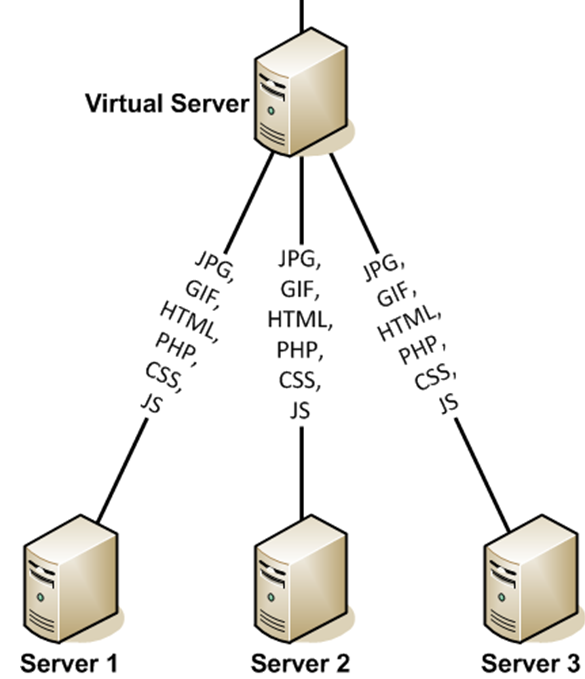
\includegraphics[width=0.5\linewidth]{images/Grafik.png}
		\caption{Ich bin eine Grafik, die eine halbe Seite groß ist und wurde dieser Onlinequelle entnommen \cite{LoadBalancing}}
		\label{Grafik}
	\end{center}
\end{figure}

